%%%%%%%%%%%%%%%%%%%%%%%%%%%%%%%%%%%%%%%%%
% University Assignment Title Page 
% LaTeX Template
% Version 1.0 (27/12/12)
%
% This template has been downloaded from:
% http://www.LaTeXTemplates.com
%
% Original author:
% WikiBooks (http://en.wikibooks.org/wiki/LaTeX/Title_Creation)
%
% License:
% CC BY-NC-SA 3.0 (http://creativecommons.org/licenses/by-nc-sa/3.0/)
% 
% Instructions for using this template:
% This title page is capable of being compiled as is. This is not useful for 
% including it in another document. To do this, you have two options: 
%
% 1) Copy/paste everything between \begin{document} and \end{document} 
% starting at \begin{titlepage} and paste this into another LaTeX file where you 
% want your title page.
% OR
% 2) Remove everything outside the \begin{titlepage} and \end{titlepage} and 
% move this file to the same directory as the LaTeX file you wish to add it to. 
% Then add \input{./title_page_1.tex} to your LaTeX file where you want your
% title page.
%
%%%%%%%%%%%%%%%%%%%%%%%%%%%%%%%%%%%%%%%%%
%\title{Title page with logo}
%----------------------------------------------------------------------------------------
%   PACKAGES AND OTHER DOCUMENT CONFIGURATIONS
%----------------------------------------------------------------------------------------

\documentclass[12pt]{article}
\usepackage[english]{babel}
\usepackage[utf8x]{inputenc}
\usepackage{amsmath}
\usepackage{graphicx}
\usepackage[colorinlistoftodos]{todonotes}

\begin{document}

\begin{titlepage}

\newcommand{\HRule}{\rule{\linewidth}{0.5mm}} % Defines a new command for the horizontal lines, change thickness here

\center % Center everything on the page
 
%----------------------------------------------------------------------------------------
%   HEADING SECTIONS
%----------------------------------------------------------------------------------------

\textsc{\LARGE Dalhousie University}\\[1.5cm] % Name of your university/college
\textsc{\Large Topics in Program Comprehension}\\[0.5cm] % Major heading such as course name
\textsc{\large CSCI 6306}\\[0.5cm] % Minor heading such as course title

%----------------------------------------------------------------------------------------
%   TITLE SECTION
%----------------------------------------------------------------------------------------

\HRule \\[0.4cm]
{ \huge \bfseries Architecture Extraction}\\[0.4cm] % Title of your document
\HRule \\[1.5cm]
 
%----------------------------------------------------------------------------------------
%   AUTHOR SECTION
%----------------------------------------------------------------------------------------

~
%\begin{minipage}{0.4\textwidth}
%\begin{flushright} \large
\emph{Group : Something} \\
Bhupendra \textsc{Rajawat} \\
Bryan Thomas \textsc{D'silva}\\ % Supervisor's Name 
Saurabh \textsc{Singh}\\
\bigskip
%\end{flushright}
%\end{minipage}\\[2cm]

% If you don't want a supervisor, uncomment the two lines below and remove the section above
%\Large \emph{Author:}\\
%John \textsc{Smith}\\[3cm] % Your name

%----------------------------------------------------------------------------------------
%   DATE SECTION
%----------------------------------------------------------------------------------------

{\large \today}\\[2cm] % Date, change the \today to a set date if you want to be precise

%----------------------------------------------------------------------------------------
%   LOGO SECTION
%----------------------------------------------------------------------------------------


\includegraphics[width=0.7\textwidth]{dal.jpg}% Include a department/university logo - this will require the graphicx package
 
%----------------------------------------------------------------------------------------

\vfill % Fill the rest of the page with whitespace

\end{titlepage}
\tableofcontents
\newpage
\begin{abstract}
Your abstract.
\end{abstract}

\section{Finding a Software System}
We looked at the following software systems and games.
\begin{enumerate}
\item \textbf{Kodi}: Kodi is an open source software media player and entertainment hub. This is available on atleast seven platforms. This was one of the first softwares we looked at and kept it as a contender

\item \textbf{Quake III}: The source code for Quake is challenging and interesting. However, there is almost no documentation for the same and hence we decided not to go ahead with this for now.

\item \textbf{GIMP}: GIMP is a cross platform image editor with an excellent community backing it up. We decided to extract the architecture for GIMP. We talk more about GIMP in the further sections.

\end{enumerate}

We also looked at Doom3, SuperTuxKart, Wordpress, TuxRunner and Linux but found GIMP to be the most interesting on to use for this assignment
\section{About GIMP}
Gimp was designed initially as a General image manipulation program. This was later changed to GNU Image Manipulation Program. It is free and openly available to retouch and edit images, convert image formats and more specialized tasks targeted towards image manipulation. GIMP provides an interface to handle simple graphics needs without learning advanced methods for image manipulation. GIMP is more user friendly as compared to other photoshop techniques and can be modified to fit your needs. And the best part about it is that it is free.
\section{Counting the lines of code}
\subsection{Count Lines of Code}
Count Lines of Code, abbreviated as CLOC is a software used to count comment lines, blank lines and physical lines of code\cite{gitid}. We used this software initially when we looked at what software system we need to pick. We can look at figure \ref{fig:clocgimp} for the output for GIMP.
\begin{figure}
\centering
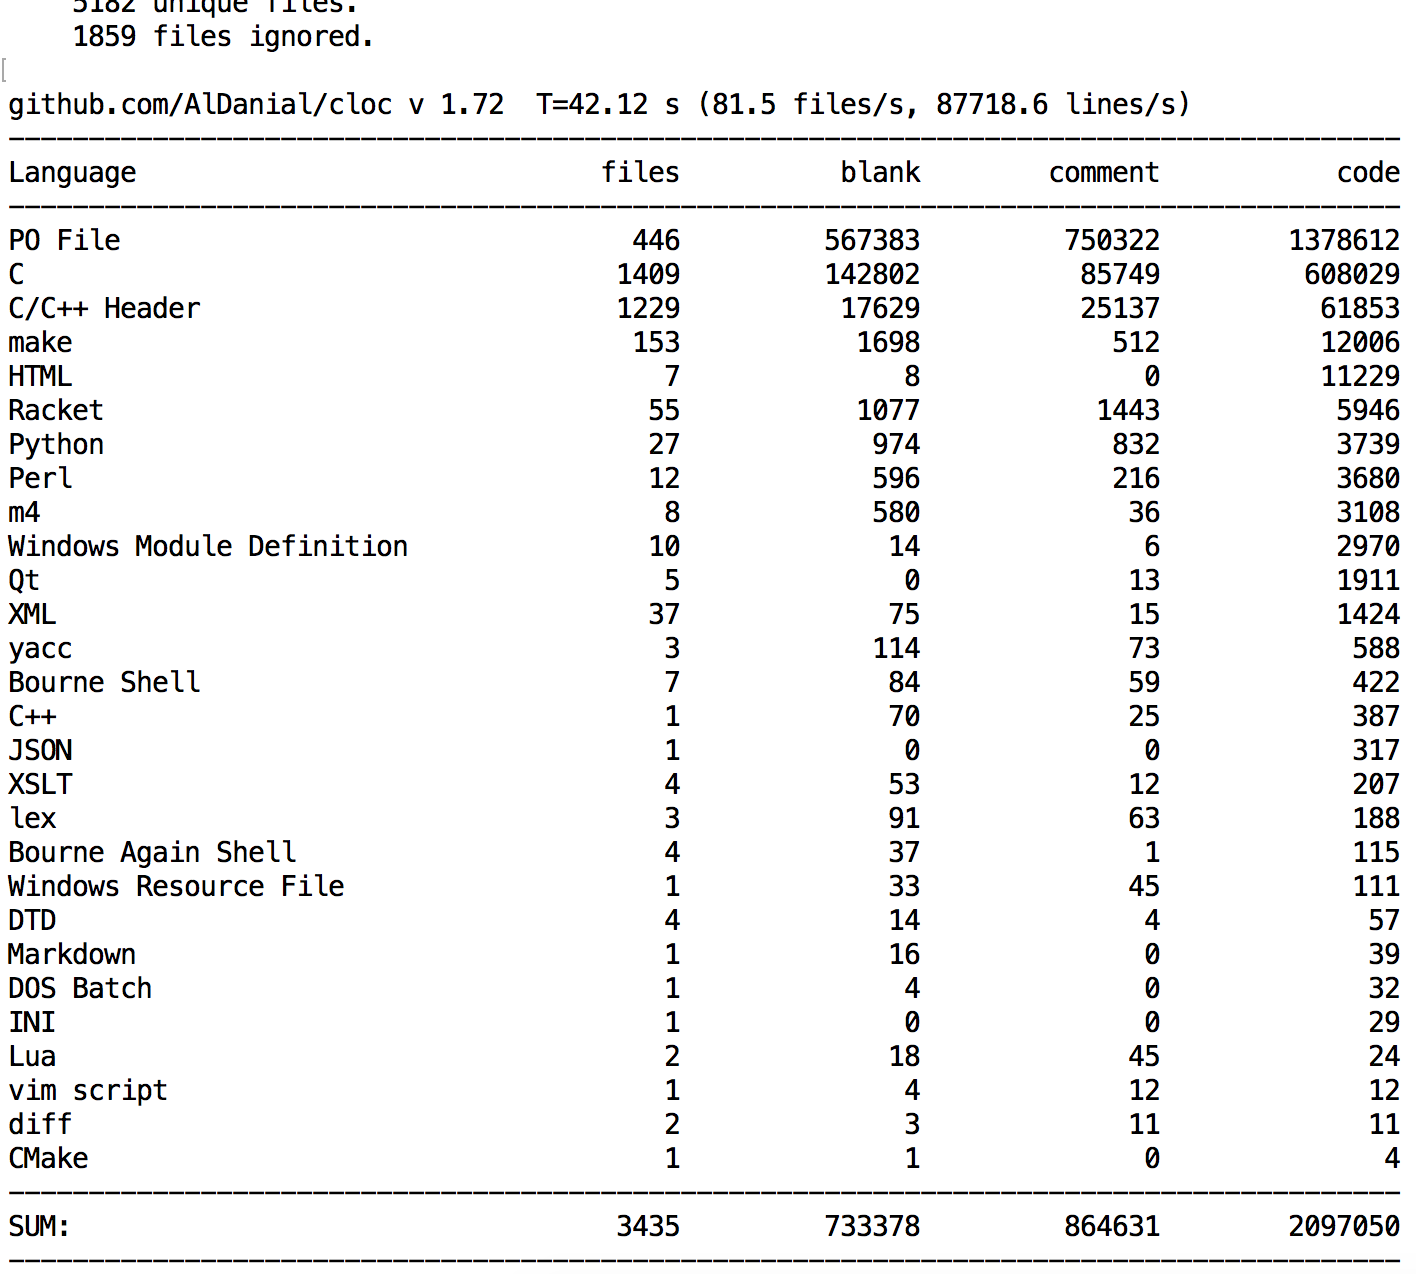
\includegraphics[width=1\textwidth]{clocgimp.png}
\caption{\label{fig:clocgimp}CLOC output for GIMP}
\end{figure}
%LocMetrics
\subsection{LocMetrics}
LocMetrics\cite{locmetrics} is very similar to what CLOC does. We did find this software interesting because of how it visualized the output.

\section{Directory Structure}
\section{Entry Point}
\section{Build Process}
\section{Control Flow}
\section{Dependencies}
\section{Functional Needs}
\section{Algorithms}
To find the underlying algorithms behind the operations performed on gimp, the wiki for the same had a link to the algorithms used. We expected to find all the underlying algorithms here but encountered a problem. There was only one operation described here shown in figure \ref{fig:algorithm}.

\begin{figure}
\centering
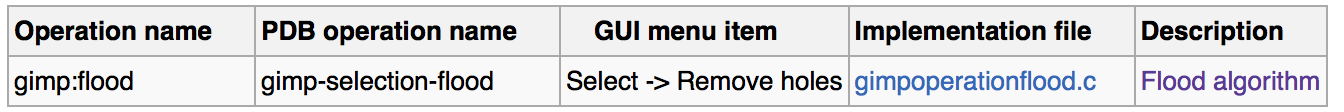
\includegraphics[width=1\textwidth]{algorithm.png}
\caption{\label{fig:algorithm}Documentation on operation algorithms}
\end{figure}

Since this is implemented in the gimpoperationflood.c, the best way to find the algorithms for the other operations performed would be to have a look at where this file is located.
 
The app/operations folder is where this file located. Looking at the other files in the folder, we got an idea of where to look incase we had to change or add any further operations. Since these operations are triggered using the GUI, changing something here would cause us to look at the UI elements to be updated as well.

\section{Conclusion}
\section{Some \LaTeX{} Examples}
\label{sec:examples}
\subsection{Sections}

Use section and subsection commands to organize your document. \LaTeX{} handles all the formatting and numbering automatically. Use ref and label commands for cross-references.

\subsection{Comments}

Comments can be added to the margins of the document using the \todo{Here's a comment in the margin!} todo command, as shown in the example on the right. You can also add inline comments too:

\todo[inline, color=green!40]{This is an inline comment.}

\subsection{Tables and Figures}

Use the table and tabular commands for basic tables --- see Table~\ref{tab:widgets}, for example. You can upload a figure (JPEG, PNG or PDF) using the files menu. To include it in your document, use the includegraphics command as in the code for Figure~\ref{fig:frog} below.

% Commands to include a figure:
\begin{figure}
\centering

\includegraphics[width=0.1\textwidth]{dal.jpg}
\caption{\label{fig:frog}This is a figure caption.}
\end{figure}

\begin{table}
\centering
\begin{tabular}{l|r}
Item & Quantity \\\hline
Widgets & 42 \\
Gadgets & 13
\end{tabular}
\caption{\label{tab:widgets}An example table.}
\end{table}

\subsection{Mathematics}

\LaTeX{} is great at typesetting mathematics. Let $X_1, X_2, \ldots, X_n$ be a sequence of independent and identically distributed random variables with $\text{E}[X_i] = \mu$ and $\text{Var}[X_i] = \sigma^2 < \infty$, and let
$$S_n = \frac{X_1 + X_2 + \cdots + X_n}{n}
      = \frac{1}{n}\sum_{i}^{n} X_i$$
denote their mean. Then as $n$ approaches infinity, the random variables $\sqrt{n}(S_n - \mu)$ converge in distribution to a normal $\mathcal{N}(0, \sigma^2)$.

\subsection{Lists}

You can make lists with automatic numbering \dots

\begin{enumerate}
\item Like this,
\item and like this.
\end{enumerate}
\dots or bullet points \dots
\begin{itemize}
\item Like this,
\item and like this.
\end{itemize}

We hope you find write\LaTeX\ useful, and please let us know if you have any feedback using the help menu above.
\bibliography{assignment}
\bibliographystyle{plain} 
\end{document}